\chapter{Zatvorene inovacije}

Zatvorene inovacije su pristup inoviranju koji se temelji na razvoju novih
proizvoda, procesa i tehnologija unutar same tvrtke, bez uključivanja vanjskih
stručnjaka, organizacija ili pojedinaca. Ovaj pristup se obično koristi u
tvrtkama koje posjeduju bogato unutarnje znanje i resurse potrebne za razvoj
novih proizvoda ili procesa \citep{zatvorenaotvorena2020,openinnovation2003}.

Zatvorene inovacije su bile dominantan pristup inoviranju u prošlosti. Većina
tvrtka u SAD-u se koristili modelom zatvorenih inovacija većinom dvadesetog
stoljeća. Model zatvorenih inovacija je doveo do puno važnih postignuća i
komercijalnih uspjeha. Zbog prijašnjih uspjeha model zatvorenih inovacija mnoge
tvrtke su nastavile koristiti ovaj pristup inoviranju i danas. Model zatvorenih
inovacija se može vidjeti u primjeni industrijama gdje su poslovne tajne jako
bitne. Primjeri takvih industrija su industrija lijekova i industrija
mikroprocesora.


Tvrtke koje primjenjuju zatvoreni pristup inoviranju obično imaju stroge interne
procese koji se koriste za generiranje novih ideja i razvoj novih proizvoda. Ove
tvrtke mogu koristiti različite metode, kao što su fokus grupe, istraživanja
tržišta i interne istraživačke timove, kako bi generirale nove ideje
\citep{zatvorenaotvorena2020,openinnovation2003}.

Zatvoreni pristup inoviranju je učinkovit pod sljedećim pretpostavkama:
\begin{itemize}
    \item tvrtka ima dovoljno znanja i resursa za razvoj novih proizvoda i usluga,
    \item tvrtka zapošljava stručnjake koji mogu razviti nove proizvode i usluge (\it{svi pametni rade za nas}),
    \item tvrtka cijeli proces razvoja novih proizvoda i usluga kontrolira i nadzire,
    \item tvrtka cijeli proces istraživanja i razvoja novih proizvoda i usluga provodi samostalno,
    \item tvrtka čuva svoje tajne i ne dijeli svoje znanje s drugim tvrtkama \citep{zatvorenaotvorena2020,openinnovation2003}.
\end{itemize}

Kod istraživanja i razvoja novih proizvoda i usluga zatvorenim pristupom broj
ideja na početku procesa je velik, a broj ideja na kraju procesa je manji. Takav
efekt se naziva efektom lijevka. Efekt lijevka je prikazan na
slici~\ref{fig:closed_inovations_funnel}. Unutar lijevka ideje prolaze kroz
različite faze razvoja, od ideje do razvoja proizvoda. U svakoj fazi razvoja
ideja se filtrira, tako da se na kraju procesa ostane samo nekoliko ideja koje
su razvijene do kraja \citep{zatvorenaotvorena2020,openinnovation2003}.

\begin{figure} 
    \centering
    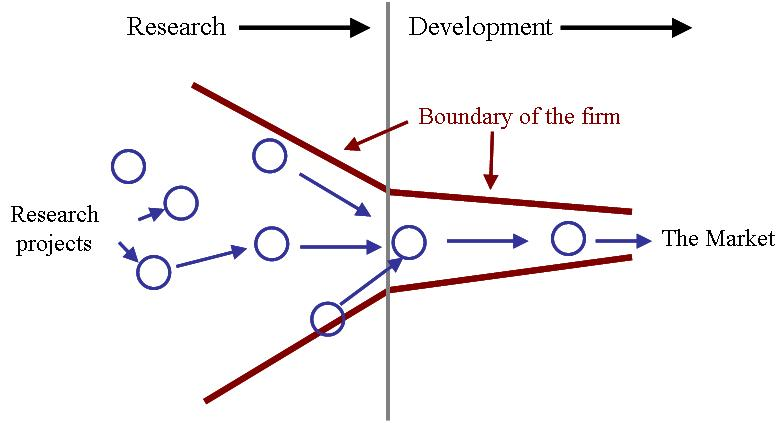
\includegraphics[width=0.8\textwidth]{images/closed_inovations_funnel.jpg}
    \caption{Zatvoreni pristup inoviranju \citep{openinnovation2016}.}\label{fig:closed_inovations_funnel}
\end{figure}

Kao posljedica efekta lijevka mnoge ideje ostanu neiskorištene, ali se dodaju u
bazu znanja tvrtke. Tvrtke koje primjenjuju zatvoreni pristup inoviranju obično
imaju veliku bazu znanja, koja se može koristiti za razvoj novih proizvoda i
usluga \citep{zatvorenaotvorena2020,openinnovation2003}.

Istraživanje i razvoj novih proizvoda i usluga rade dvije skupine ljudi:
\begin{itemize}
    \item istraživači koji razvijaju nove ideje i
    \item inženjeri koji razvijaju nove proizvode i usluge.
\end{itemize}
Istraživači su najčešće jako specijalizirani znanstvenici ili inženjeri,
najčešće s doktoratom. Tvrtke ih vrbuju velikim plaćama i velikom slobodom rada
na projektima. Pošto su istraživači jako specijalizirani teško ih je ponovno
trenirati ako se poslovno stanje promijeni. Inženjeri na drugoj strani su
specijalizirani za rješavanje problema unutar zadanih granica. Uzimaju rezultat
istraživanja i razvijaju proizvod ili uslugu unutar zadanih granica, vrijeme i
budžet \citep{openinnovation2003}.